\documentclass[tikz]{standalone}
\begin{document}

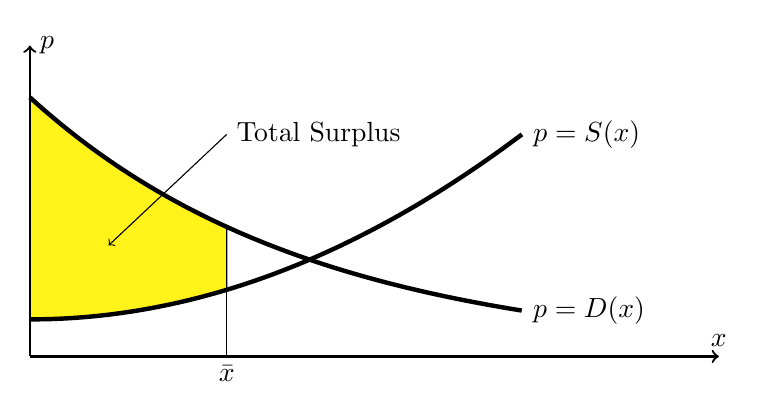
\begin{tikzpicture}[xscale=2.5,yscale=0.94]

  % shade region
  \draw[fill=yellow!90] plot[smooth, samples=10, domain=0:1] (\x,3.5/2^\x) -- 
  plot[smooth, samples=100, domain=1:0] (\x,0.5+0.4*\x*\x);

  % draw axes 
  \draw[thick,->] (0,0) -- (3.5,0) node[above] {$x$};
  \draw[thick,->] (0,0) -- (0,4.2) node[right] {$p$};
    
  % draw curves
  \draw[ultra thick,domain=0:2.5,samples = 100, smooth,variable=\x,black] plot ({\x},{3.5/2^\x})node[right] {$p=D(x)$};
  \draw[ultra thick,domain=0:2.5,smooth,variable=\x,black] plot ({\x},{0.5+0.4*\x*\x}) node[right] {$p=S(x)$};

  % draw labels
  \draw (1,0.9) -- (1,0) node[below] {$\bar{x}$};
  \draw[<-] (0.4,1.5) -- (1,3) node[right] {Total Surplus};
\end{tikzpicture}
\end{document} 
